\chapter{Psalm 7}


\begin{figure}
  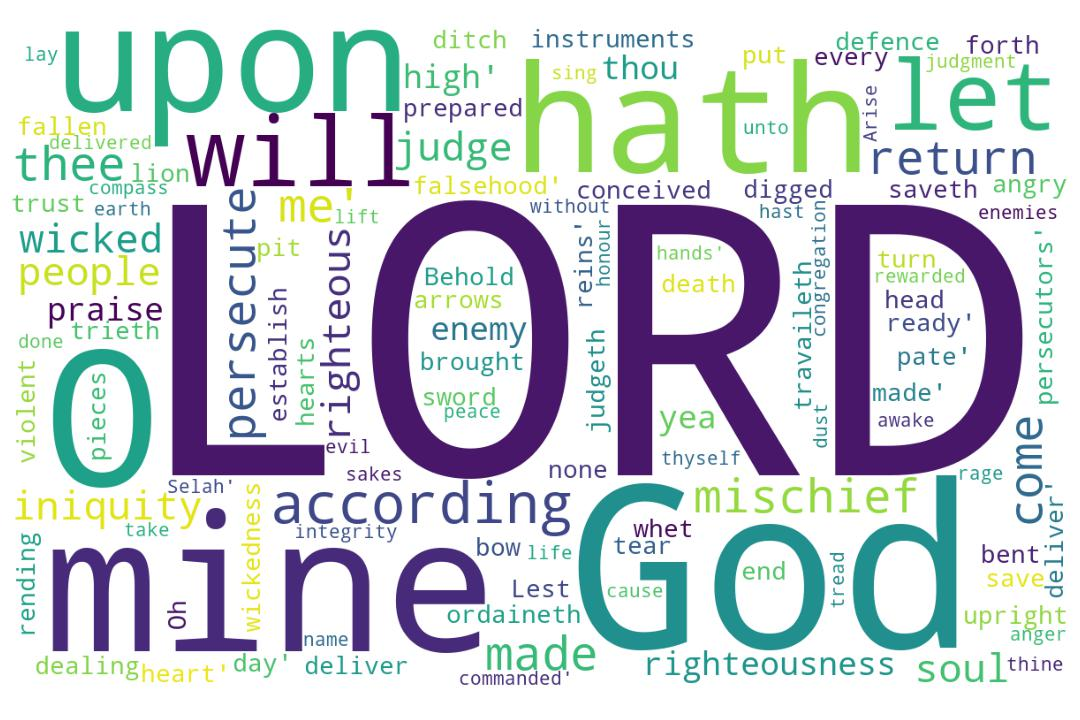
\includegraphics[width=\linewidth]{19OT-Psalms/Psalm7-WordCloud.jpg}
  \caption{Psalm 7 Word Cloud}
  \label{fig:Psalm 7 word Cloud}
\end{figure}



\marginpar{\scriptsize \centering \fcolorbox{bone}{lime}{\textbf{ABOUT DISTRESS}}\\
 \fcolorbox{bone}{lime}{\textbf{\& DELIVERANCE}} \\ (Psalm 7:1-17) \begin{compactenum}[I.][8]
    \item \textbf{Recognizes Sin and its Damage}
    \item \textbf{Reaches a State of Despair}
    \item \textbf{Remembers the Source of his Deliverance}
    \item \textbf{Repeats his Sorrow and Distress}
    \item \textbf{Recounts the Sum of Adversaries}
    \item \textbf{Requests Sinners to Departs}
    \item \textbf{Rejoices in his Savior and Deliverer}
\end{compactenum}}

\marginpar{\scriptsize \centering \fcolorbox{bone}{yellow}{\textbf{ACCUSED}}\\
 \fcolorbox{bone}{yellow}{\textbf{\& APPEALING}} \\ (Psalm 7:1-17) \begin{compactenum}[I.][8]
    \item The \textbf{First Appeal} \index[scripture]{Psalms!Psa 007:001} (Psa 7:1)
    \item A \textbf{False Accusation} \index[scripture]{Psalms!Psa 007:003} (Psa 7:3)
    \item \textbf{Fitting Amends} \index[scripture]{Psalms!Psa 007:005} (Psa 7:5)
    \item \textbf{Fierce Anger} \index[scripture]{Psalms!Psa 007:006} (Psa 7:6)
    \item A \textbf{Final Accounting} \index[scripture]{Psalms!Psa 007:008} (Psa 7:8)
    \item \textbf{Full Assurance} \index[scripture]{Psalms!Psa 007:010} (Psa 7:10)
    \item The \textbf{Final Annihilation} \index[scripture]{Psalms!Psa 007:016} (Psa 7:16)
\end{compactenum}}

\footnote{\textcolor[cmyk]{0.99998,1,0,0}{\hyperlink{TOC}{Return to end of Table of Contents.}}}\footnote{\href{https://audiobible.com/bible/bible.html}{\textcolor[cmyk]{0.99998,1,0,0}{Psalms Audio}}}\textcolor[cmyk]{0.99998,1,0,0}{Shiggaion of David, which he sang unto the LORD, concerning the words of Cush the Benjamite.}\\
\\
\textcolor[cmyk]{0.99998,1,0,0}{O\textcolor{jungle}{$_{1131}$} LORD my God, in thee do I put my trust: save me from all them that persecute me, and deliver me:}
[2] \textcolor[cmyk]{0.99998,1,0,0}{Lest\textcolor{jungle}{$_{1153}$} he tear my soul like a lion, rending \emph{it} in pieces, while \emph{there} \emph{is} none to deliver.}
[3] \textcolor[cmyk]{0.99998,1,0,0}{O\textcolor{jungle}{$_{1171}$} LORD my God, if I have done this; if there be iniquity in my hands;}
[4] \textcolor[cmyk]{0.99998,1,0,0}{If\textcolor{jungle}{$_{1187}$} I have rewarded evil unto him that was at peace with me; (yea, I have delivered him that without cause is mine enemy:)}
[5] \textcolor[cmyk]{0.99998,1,0,0}{Let\textcolor{jungle}{$_{1211}$} the enemy persecute my soul, and take \emph{it}; yea, let him tread down my life upon the earth, and lay mine honour in the dust. Selah.}
[6] \textcolor[cmyk]{0.99998,1,0,0}{Arise\textcolor{jungle}{$_{1238}$}, O LORD, in thine anger, lift up thyself because of the rage of mine enemies: and awake for me \emph{to} the judgment \emph{that} thou hast commanded.}
[7] \textcolor[cmyk]{0.99998,1,0,0}{So\textcolor{jungle}{$_{1265}$} shall the congregation of the people compass thee about: for their sakes therefore return thou on high.}
[8] \textcolor[cmyk]{0.99998,1,0,0}{The\textcolor{jungle}{$_{1283}$} LORD shall judge the people: judge me, O LORD, according to my righteousness, and according to mine integrity \emph{that} \emph{is} in me.}
[9] \textcolor[cmyk]{0.99998,1,0,0}{Oh\textcolor{jungle}{$_{1306}$} let the wickedness of the wicked come to an end; but establish the just: for the righteous God trieth the hearts and reins.}
[10] \textcolor[cmyk]{0.99998,1,0,0}{My\textcolor{jungle}{$_{1330}$} defence \emph{is} of God, which saveth the upright in heart.}
[11] \textcolor[cmyk]{0.99998,1,0,0}{God\textcolor{jungle}{$_{1341}$} judgeth the righteous, and God is angry \emph{with} \emph{the} \emph{wicked} every day.}
[12] \textcolor[cmyk]{0.99998,1,0,0}{If\textcolor{jungle}{$_{1354}$} he turn not, he will whet his sword; he hath bent his bow, and made it ready.}
[13] \textcolor[cmyk]{0.99998,1,0,0}{He\textcolor{jungle}{$_{1372}$} hath also prepared for him the instruments of death; he ordaineth his arrows against the persecutors.}
[14] \textcolor[cmyk]{0.99998,1,0,0}{Behold\textcolor{jungle}{$_{1389}$}, he travaileth with iniquity, and hath conceived mischief, and brought forth falsehood.}
[15] \textcolor[cmyk]{0.99998,1,0,0}{He\textcolor{jungle}{$_{1402}$} made a pit, and digged it, and is fallen into the ditch \emph{which} he made.}
[16] \textcolor[cmyk]{0.99998,1,0,0}{His\textcolor{jungle}{$_{1418}$} mischief shall return upon his own head, and his violent dealing shall come down upon his own pate.}\footnote{\textbf{Genesis 3:15} - And I will put enmity between thee and the woman, and between thy seed and her seed; it shall bruise thy head, and thou shalt bruise his heel.}
[17] \textcolor[cmyk]{0.99998,1,0,0}{I\textcolor{jungle}{$_{1437}$} will praise the LORD according to his righteousness: and will sing praise to the name of the LORD most high\textcolor{jungle}{$_{1457}$}.}

